%!TEX root = kudzai_thesis.tex
%%%%%%%%%%%%%%%%%%%%%%%%%%%%%%%%%%%%%%%%%%%%%%%%%%%%%%%%%%%%%%%%%%%%%%%


\chapter{Problem Statement}


Mass demonstrations by people often result in vandalism of public property in industry, academia, etc., which leads to the disruption of daily organizational activities.
They often use social media as a platform to express their views, sometimes extreme views towards the authorities. Opinions expressed by people can give very valuable information assisting in the decision-making process. Nowadays several websites encourage users to express and exchange their views, suggestions and opinions related to textual content publicly. The increase in popularity of these sites resulted in huge collection of people's opinions on the web in much unstructured manner. Drawing insights from the opinion sources is a challenging task. Recent attempts to compute sentiment analysis on unstructured data have used techniques such as opinion mining and sentiment lexicons.


\section{Objectives}
To achieve the aim of the study the following objectives have been drawn. 
\begin{itemize}
\item To detect people\textquotesingle s mood from textual information posted on social media.
\item To classify people\textquotesingle s sentiment based on their geographical location.
\end{itemize}

\section{Aim}

Our aim is to develop a system that can classify people\textquotesingle s mood and sentiment based on the textual information they post on social media.



\section{Significance of the Study}
Leaders of today face many difficult, potentially explosive situations in which they must make decisions that can help or harm their firms, themselves or others. Sentiment analysis will improve the ethical quality of decisions made by the authorities and managers, and also ensure that decisions made will not backfire. It also helps the authorities to predict the outcome of the decisions made, and determine the impact on the affected population. This study helps us to evaluate the degree of evaluability/argumentativeness with which the population under study communicates, and make improved decisions drawn from insights on the analyzed data.



\chapter{Research methodology}
\section{Sentiment Analysis process}
A graphical description of the processes involved in sentiment analysis approach that this research will follow is detailed in the diagram shown below:

\begin{figure}[h]
  \centering
  \pgfimage[width=0.7\linewidth]{images/research_methodology}
  \caption[Sentiment analysis process]
  {Basic processes involved in sentiment analysis, source:\cite{ref14}}
  \label{fig:ALAP:sm3}
\end{figure}
\label{research_methodology}


\subsection{Data Collection}
Sentiment analysis harnesses the huge amount of content generated over the internet. Some data sources of the content are public forums, product review sites, blogs, discussion boards and social networking sites like Twitter and Facebook.
The data is produced rapidly and is often bulky and unstructured.

Because people will express their emotions differently with regards to choice of language and style of writing, some may prefer to use slang and emoticons to name a few. This means that manually analyzing this text is a tedious and an almost impossible task.
\clearpage
However, with sentiment analysis, we can make use of natural language processing techniques to filter the useful information for analysis and classify it accordingly. An example of the type of data is presented below



\begin{figure}[h]
  \centering
  \pgfimage[width=0.8\linewidth]{images/sample_tweets}
  \caption[sample tweets]
  {Data extracted from online sources Source: \url{http://www.sentiment140.com/search?query=CocaCola&hl=en}  }
  \label{fig:ALAP:sm1}
\end{figure}



\subsection{Text Preparation}
The text preparation process begins by cleaning the textual data prior to the analysis stage. Normally text preparation involves identifying and removing non textual content from the data such as hash tags and hyperlinks. Also, some non-essential information that does not contribute to the reviewer's opinion such as name and location and date all these are removed, also any other content that is deemed irrelevant to the analysis is also removed.

\subsection{Sentiment Detection}
Stage 3 of fig \ref{research_methodology}, detecting sentiment, involves extracting the opinions from the reviews by the use of textual processing. The textual data is broken down into sentences and each sentence is analyzed for subjectivity. Sentences that are not subjective are discarded, only those that contain subjective text are kept for further analysis. Next sentiment detection is done, and it can either be done on single term level, phrase level, sentence or document level. Some of the techniques used are

\begin{itemize}

\item \textbf{Unigrams:} Also known as a bag of word technique, whereby each element will be represented as a feature vector based on the frequency of a single word.

\item \textbf{N-Grams:} This is an approach that represents features of a document by a number of words in a specific sequence, for example, words in pairs or triplets... etc. up to "N" hence N-gram

\item \textbf{Lemmas:} Lemmatization is a process whereby words are converted to their synonyms instead of using the literal word, and example of lemmatization is\\
better $\xrightarrow{}$ good, best $\xrightarrow{}$ good.\\
This approach makes better generalization and simplifies the process of analysis.

\item \textbf{Negation:} This method works in a much similar way to n-grams method, such phrases like “I like this book” and “I do not like this book”, using other techniques can be classified as being in the same category, but with negation included the two phrases are in opposite classes. However, negation cannot work in all situations, such as when sarcasm or satire is used \cite{ref19}. Also, the polarity is not always reversed when negation is detected.

\item \textbf{Opinion words:} When people express their emotions they often use, "feeling words" these can be adjective and adverbs. Words like these can be incorporated into a feature vector and they can represent the proximity of a word to a similar word, this is a good way to detect subjectivity in a document.
\end{itemize}

\subsection{Sentiment Classification}
Stage 4 of the analysis stage is polarity detection, which will classify each of the subjective sentences into the classification groups, usually binary positive or negative but sometimes can also be neutral.

Some basic techniques of supervised learning for classification are:
\begin{itemize}
\item Naive Bayes (NB)
\item Support vector machines (SVM)
\item Maximum entropy (ME)
\end{itemize}
The NB classifier is a probabilistic classifier which works by applying Bayes theorem.
Support vector machines are based on the statistical learning theory, it looks for a hyper plane that maximizes the distance between a binary class.

The ME model is constructed from features which correspond to some constraint on the model, then the model which has the maximum entropy is selected as the class.

\clearpage
\subsection{Presentation of Output}
The main aim of the analysis is converting a huge volume of unstructured textual data into insights. When the analysis is completed, many visual techniques can be used to display the results of the analysis, such as pie charts, bar graphs and line graphs, the information can be displayed in a continuous stream as the data is analyzed in real time it is being displayed.\\

An example is shown below:

\begin{figure}[h]
  \centering
  \pgfimage[width=0.7\linewidth]{images/sentiment_summary}
  \caption[example of sentiment analysis results]%
  {Sentiment analysis results summary Source: http://www.sentiment140.com/ }
  \label{fig:ALAP:sm3}
\end{figure}




\section{Limitations}
Due to the limitations of the current information processing and analysis techniques ( i.e. search
engines cannot crawl and process pictures, video, flash, executive scripts, executive program and
other non-text content files ), images, videos, folders, executive files, package files and other
online transmission information and data are not included in our analysis, \cite{ref22}.


\leavevmode\\
When a major geopolitical event takes place and news of it spreads on the internet. Mass media and reports stirs up comments on social media which can effectively reflect the sentiment of the majority of the citizens. But as it is difficult to do extensive gathering and analysis of ancillary data and theme events, information to reveal and explain the spatial diffusion of internet attention always be blocked and insipid, \cite{ref22}. As a result, this study will use the twitter API to gather textual information based on a geographic location, to detect moods of a particular population on a certain topic.


\subsection{Delimitation of the study}
Although there may be value in studying all social network platforms and mass media sites, this study is limited to Twitter comments. One of the complicating factors when doing online sentiment detection 
is the fact that most people often ignore the rules and spellings of grammar, this factor my affect the quality of the analysis.


\section{Literature Review}
\subsection{Overview}
In the following chapter we explore available technologies as well as progress that has been achieved in sentiment analysis. We  will discuss the work that is related to the existing work that has been done and the contributions made. This chapter also reviews the relevant literature and establishes the research framework for the study. We review several approaches adopted to perform basic computational analysis of sentiments and opinions. Various techniques to Sentiment Analysis like Naïve Bayes, Maximum Entropy, and Support Vector Machine will be discussed and their strengths and weaknesses will be examined.


\subsection{Sentiment Analysis}
Sentiment analysis is also known as opinion mining, it aims to detect subjective text and extract useful information from given textual data. The text can be classified as binary positive or negative but sometimes also neutral. 
By making use of techniques and mechanisms insights can be drawn from the textual information. A huge corpus of textual data can be ingested into a statistical model and processed to produce information that can support operational, managerial, and strategic decision making \cite{ref6}. In addition, sentiment analysis is a tool in data mining that can overcome challenges like harnessing, analyzing and interpreting textual content since data is dispersed, disorganized, and fragmented by systematically extracting and analyzing online data without facing any time delays \cite{ref7}.
\leavevmode\\

Natural language processing (NLP) approaches, are able to capture the specificity of sentiment nuances through a variety of concepts, like part-of-speech disambiguation, sentence parsing, entity extraction, and context-based Boolean operators. They usually involve a form of rule-writing, which requires up-front manual labor but, once developed enables the desired accuracy levels within the subjective context.
\leavevmode\\

Sentiment analysis is arguably the fastest growing areas of research in NLP. The growth of social media platforms such as online reviews has also resulted in the growth in importance of sentiment analysis, forum discussions, blogs, micro-blogs, Twitter, and social networks has increased the need to study this area. \cite{ref20}. Because of the vast amount of opinionated data that the web holds, if properly analyzed this can drastically help businesses and policy makers in their decision making. Using text mining and analysis techniques such as Artificial Neural Network (ANN) and Support Vector Machine (SVM), classification of sentiments can easily be performed even in real time.
\leavevmode\\

In particular, Twitter has become the top social media analytics channel due to its simple to use API, and social impact by some influential people, politicians and celebrities. With over 3 billion tweets and 15 billion Application Programming Interface (API) calls generated daily \cite{ref8}. Twitter has both the supply and demand for opinionated data for a wide range of topics. One of the reasons for Twitter's rapid growth in demand is because of the growing number of social media analytic applications  that make use of twitter's API. A major aspect of Twitter is Twitter sentiments, which are harnessed for understanding customer behavior and preferences \cite{ref11}, predicting financial performance \cite{ref9}, providing early warnings for undesirable medical catastrophes \cite{ref10}, predicting and understanding election outcomes, and as archived data which can potentially be used in the future for disaster response and surveillance systems \cite{ref13}, etc. Several sentiment search engines exist where users run typical queries on any topic of interest, and generate text results. The results are normally classified into 3 polar categories, positive, neutral and negative. Some examples currently available are \cite{ref14},

\begin{itemize}

\item They Say IO:  http://www.theysay.io
\item Text2Data:  https://text2data.com/
\item Summerizebot:  https://www.summarizebot.com
\item Sentiment140: http://www.sentiment140.com/
\item Parallel dots: https://www.paralleldots.com/

\end{itemize}
\leavevmode\\
Looking at how data on twitter is analyzed, a certain tool is used for sentiment analysis which is called the Sentimentor. It makes use of the naive Bayes Classifier to categorize tweets into one of three classes, negative, neutral or positive classes. Sentimentor's user interface has an allows the user to visually analyze the word distributions. This tool presents classification results in an easy to understand pictorial format. Other insights drawn by Sentimentor include, the type of text and details of analysis \cite{ref15}.

\leavevmode\\
The majority of opinion mining tools aim to detect the polarity of a textual document, they classify the polarity as either positive, negative, or neutral. For many applications this is sufficient, but textual data often contains a mix of sentiment both positive and negative in the same document, so at times it is necessary to be able to detect both simultaneously and also to determine the intensity of the sentiment expressed. An example may be programs that are used to monitor online chat rooms, and screen for inappropriate language or tone which could put other users at risk \cite{ref16}, must be able to detect both the strength and polarity of the information or sentiment expressed and whether participants were appropriately balancing positive and negative sentiment. Additionally some research to explore the role emotions play in online communication \cite{ref17}, can benefit from opinion mining, as would the growing body of psychology and other social science research into the role of sentiment in various types of discussion or general discourse \cite{ref18}.

\clearpage
An institution can enhance the decision making of its executive board by the simple use of Sentiment Analysis and machine learning Techniques. This research project is based on the design of an integrated system that will perform the semantics or text analysis. This project will consider the analysis, design and implementation of machine learning algorithms to demonstrate sentiment analysis on textual content of an event \cite{ref19}.
Recently we are starting to see an emergence of tools that can analyze sentiment at a feature level, but in general automated sentiment analysis technology has difficulty discerning one topic from another more so if many topics are discussed in the same document.
\leavevmode\\


\subsection{Related work}
As previously defined sentiment analysis aims to harness the vast amount of user generated data online. 
Some of the main characteristics of such data is its high velocity, high volume and textual disorder as well as its diversity. 
Computational linguistic is a field in NLP and is used to detect, extract and analyze subjective textual information from a given document. 
The main aim is to extract the writer's opinion towards a given topic or to get the overall contextual polarity of the document.
Most of the sentiment analysis tools that were developed long ago and that are still being developed
recently use machine learning algorithms or techniques as a way of solving different kind of
problems in developing sentiment analysis tools. There are two main ways to calculate sentiment
based on given text.


\subsection{Computation Science Techniques}
Sentiment analysis of digital texts uses machine learning e.g.  SVM, bag-of-words model and Naive Bayes.
\cite{ref26}. Computational statistics refers to computationally intensive statistical methods
including re-sampling methods, Markov chain Monte Carlo methods, local regression, kernel
density estimation and principal components analysis. 

Machine Learning aims to automate processing huge amounts of data with many variables. Machine learning is commonly used in areas such as pattern recognition for speech and  images
in medicine for tumor detection and drug discovery, in finance for financial algorithms, credit scoring and algorithmic trading, for energy use forecasting and determining the load and predicting price.
Two machine learning techniques are illustrated in the diagram below:


\begin{figure}[h]
  \centering
  \pgfimage[width=0.7\linewidth]{images/machine_learning_types}
  \caption[Machine learning types]%
  {Machine Learning Types: Source: \cite{ref49}}
  \label{fig:ALAP:sm3}
\end{figure}


\clearpage
\subsection{Machine Learning Types}

Machine learning can be defined as system capable of the autonomous acquisition and integration of knowledge learned from experience [Murphy, 2012].
These systems can be subdivided into:
\leavevmode\\
\textbf{a) Supervised learning}\\
Examples of supervised learning include: Discriminant Function Analysis, Support Vector Machines, Regression Trees.\\
\textbf{b) Unsupervised learning}\\
Unsupervised learning techniques include Self-Organizing Maps (SOM), K-Means clustering.
In unsupervised learning the model is fed information but is expected to figure out information without any guidance.
\leavevmode\\

\subsection{Examples of Machine Learning Algorithms}
Machine learning algorithms make use of scientific principles that learn and help in classifying sentiment from given data. The algorithms are based on models built from inputs and validated on training data, they can then be used in making predictions based on this information, this method of generalizing is a better approach instead of following explicitly programmed instructions. Naïve Bayes Classifier (supervised) Are a group of probabilistic classifiers based on applying Bayes’ theorem with strong independence assumptions between the features. Naïve Bayes classifier makes use of a probabilistic model and can capture uncertainty by determining probabilities of the outcomes \cite{ref29}


\textbf{Bayes theorem states that:}
\begin{figure}[h]
  \centering
  \pgfimage[width=0.7\linewidth]{images/bayes_theorem}
  \caption[Bayes theorem]%
  {Bayes theorem}
  \label{fig:ALAP:sm3}
\end{figure}

\leavevmode\\
\noindent 
Where: the notation P (c | x) means "the probability of c given x."
To compute sentiment analysis on structured data using the naïve Bayes classifier in this case, we
want to know the probability of a given category given a certain string of words in a document.

\subsection{Maximum Entropy (supervised)}
Another probabilistic based classifier  is the Maximum Entropy (MaxEnt) classifier. It belongs to the class of
exponential models. MaxEnt does not make the assumption that the features are conditionally independent. 
The Maximum Entropy algorithm is based on the Principle of Maximum Entropy. It selects from all the models based on the training set the one model that has the largest entropy this is the class of interest \cite{ref19}


\subsection{Support Vector Machines (supervised)}
A Support Vector Machine (SVM) is a binary classifier, it separates two classes by a hyper-plane. In other words, given labelled training data (supervised learning), the algorithm
outputs an optimal hyper-plane which categorizes new examples, \cite{ref30}

\begin{figure}[h]
  \centering
  \pgfimage[width=0.5\linewidth]{images/support_vector_machine}
  \caption[Support vector machine]%
  {Support Vector machine Source:\cite{ref28}}
  \label{fig:ALAP:sm3}
\end{figure}

\clearpage
\subsection{K-Means Clustering (unsupervised)}
K-means clustering is a type of unsupervised learning that puts objects into classes. No a-priori
knowledge of which class objects belong to not necessarily any knowledge of how many classes
actually exist.

\begin{figure}[h]
  \centering
  \pgfimage[width=0.5\linewidth]{images/k_means_clustering}
  \caption[K-means clustering]%
  {Unsupervised K-Means Clustering, Source: https://towardsdatascience.com/k-means-clustering-identifying-f-r-i-e-n-d-s-in-the-world-of-strangers-695537505d}
  \label{fig:ALAP:sm3}
\end{figure}

\leavevmode\\
\section{Studies on Sentiment Analysis Using the Naïve Bayes Classifier}
Below is Andy Bromberg\textquotesingle s basic workflow for the project:
\begin{itemize}
\item Step 1: Select training set of positive and negative elements.
\item Step 2: Train the classification algorithm using the training data.
\item Step 3: Use classification algorithm to classify sample data.
\item Step 4: Compare the results against the known results set.
\end{itemize}
Methods used
Andy Bromberg\textquotesingle s method of sentiment extraction made use of a Natural Language Toolkit
(NLTK). This is a library for Python that does text processing and analysis. This was used to form
the basis for his sentiment analysis program. Python language was used because it has a number
of very useful libraries for text processing and sentiment analysis, and is also a simple programing
language. The methods employed by Andy Bromberg involve the use of statistics, machine
learning and classification algorithms, and the use of data mining techniques, \cite{ref31}

\subsection{Choosing the training set}
The data chosen to test the analysis was taken from product and movie reviews, instead of Twitter,
and the reason being was that Tweets are too varied, not only in intention but also in language.
The base content was taken from Bo Pang’s page on movie review data, and consisted of his
sentence polarity dataset v1.0, which had 10,663 sentences from movie reviews, each of which was labeled as
either negative or positive. Next, the positive and negative sentences were loaded up and split into
individual lines to be analyzed on a sentence level, the AFINN wordlist was used to train the
classifier. The AFINN wordlist has 2477 words and phrases rated from -5 [very negative] to +5
[very positive]. But the wordlist was reclassified into four categories:


\begin{center}


Very Negative (rating -5 or -4)\\
Negative (rating -3, -2, or -1)\\
Positive (rating 1, 2, or 3)\\
Very Positive (rating 4 or 5)

\end{center}

A few more words specific to movies were added to the list of training data to add more words to
the training set. Andy Bromberg\textquotesingle s model deliberately chose to ignore neutral words because he believed these would not help in the classification. The model then counted the number of words in each review that fit one of those four categories. This created a big data table (10,663 rows) of the form: \leavevmode\\
\textbf{
Sentence | \#vNeg | \#neg | \#pos | \#vPos | sentiment
}

Below is a sample extracted from the polarized data:
\begin{figure}[h]
  \centering
  \pgfimage[width=0.7\linewidth]{images/andy_sample}
  \caption[Sample training data]%
  {Sample form of training data}
  \label{fig:ALAP:sm3}
\end{figure}


In this sample, it means that sentence had 1 negative word, 3 positive words, and 1 very positive
word. It was also classified as positive by the database creator.
As mentioned earlier Andy Bromberg\textquotesingle s model made use of a machine learning algorithm called
the Naive Bayes classifier from the “e1071”  package to attempt to classify the sentences as positive
or negative.
The essential idea of the Naïve Bayes classifier is that it looks at how the number of words in each
of the four categories relates to whether the sentence is positive or negative. It attempts to make a probabilistic guess whether a sentence is positive or negative by analyzing  how many words it has in each category
and relating this to the probabilities of those numbers appearing in positive and negative sentences,
\cite{ref31}


\clearpage
\subsection{Results}

A confusion matrix was used to visualize the results of a classification algorithm. The matrix for
the result was:

\begin{figure}[h]
  \centering
  \pgfimage[width=0.5\linewidth]{images/andy_confusion_matrix}
  \caption[Confusion matrix results]%
  {Confusion matrix results, source: \cite{ref31}}
  \label{fig:ALAP:sm3}
\end{figure}


The confusion table shows a comparison between the predicted positive and negative sentiments
with the actual sentiments. The results show that the predicted scores were less than the actual
scores in both the positive sentiments. On the other hand, the predicted scores were greater than
the actual scores in the negative sentiment.

\subsection{Strengths and Challenges of this Method}
Andy Bromberg\textquotesingle s model made use of a supervised learning method (Naïve Bayes classifier), the
choice of using supervised learning enabled the model to train very fast, also because all the data
consists of labelled training data it enables the results to be easily clustered and to be compared to
the training data. However, all forms of supervised machine are domain specific. The Naïve Bayes
classifier is domain specific that means that it can only classify data in a field that it was trained
for. This is the reason why the classification results turned out to be less than 70\% accurate in most
cases, \cite{ref31}.
\leavevmode\\
According to Andy Bromberg\textquotesingle s model, the classification results were not accurate. On average, a
good classifier should get much higher than a 60-65\% correct classification rate. We suggest using
different classification algorithms, wordlists, and training data in the tool that we will develop.



\subsection{Studies on Term Frequency—Inverse Document Frequency}
\textbf{Method Used:}\\
This method can be used to determine the relevance of a comment to  a given context i.e if it is on topic. To achieve this an information retrieval method called "Term Frequency-Inverse Document Frequency" is employed.
TFIDF is a statistical model that infers the relevance of a word in a given textual context.
Though it was intended for the early search engines as a way of evaluating the relevance of a document in a query search, it's used also in modern search engines as a way to model a content query from text to be passed to a search engine to retrieve similar documents. In a way, it can be viewed as a document similarity measure. The "TFIDF" document representation technique treats each document as
a bag of words, where words have a varying degree of relevance  in the given document. The importance of a word is increased the the number of times it occurres in a document (term frequency, TF. In one study,  a corpus was formed from news stories obtained from Reuters was used to compute document frequency values


\subsection{Studies Using Lexicon-Driven Methods}
\cite{ref33} used the Multi-Perspective Question-Answering (MPQA) sentiment lexicon of \cite{ref34} to identify sentiment in tweets mentioning Barack Obama. To classify a tweet, they simply counted if it contains more positive or negative words according to the sentiment lexicon. Even though this is a very simple approach, they report significant correlation between the aggregated sentiment in tweets and public opinion polls published by Gallup. \cite{ref35} proposed a lexicon-based algorithm called SentiStrength, which assigns a binary polarity (positive/negative) and corresponding strength value between 1 and 5 to a given text. In addition to having a list of 298 positive and 465 negative terms annotated with polarity and strength values, SentiStrength uses lists of emoticons, negations and boosting words in the decision process. To address the issue of emphatic lengthening the authors proposed a 3 step procedure to reduce words to their standard form. After comparing SentiStrength to several ML classifiers based on MySpace comments, the author's method was found to perform better for classifying negative sentiment, but this is not the case for positive sentiment. The algorithm is enhanced in \cite{ref35}, where the authors introduce idiom lists and strength boosting by emphatic lengthening as well as an unsupervised version of SentiStrength. Furthermore, the number of terms in their sentiment strength wordlist was increased from 693 to 2310.They again compare their algorithm with different machine learning algorithms on six different datasets, including Twitter data, and found especially logistic regression to outperform SentiStrength \cite{ref35}

\subsection{Studies Using Graph-Based Label Propagation}
\cite{ref36} also experiment with a label propagation method and compared its performance
to popular online tools for sentiment analysis of tweets and a dictionary based approach. They
investigated the special role of emoticons in tweets and also used a graph propagation algorithm
to classify the sentiment of tweets in other languages than English \cite{ref37}



\leavevmode\\
\textbf{Methods used}\\
There are three main approaches in the previous research on sentiment analysis on Twitter. As
with sentiment analysis in general, the most popular approach is to train supervised machine
learning classifiers, either on manually annotated data or data labelled by “noisy" labels such as
emoticons. Many authors report their best results using support vector machines or a Naive Bayes
classifier. The second approach is lexicon-based methods, which assigns labels or scores to tweets
by aggregating scores found in sentiment lexica. Sometimes the aggregation simply consists of
summing or averaging over the polarity values of all words of the tweet found in the used lexicon,
while in other cases rules are used to address linguistic circumstances such as negation. The third
approach is based on label propagation methods, leveraging the connections between textual
content to assign sentiment values to closely connected data. While most research can be
categorized as one of these approaches, some studies also combine them.

\subsection{Studies on Predicting Users Actions from Sentiment}
Social media users often have specific sentiment towards for example, ongoing campaigns and
take different actions based on their sentiments. \cite{ref38}, presents an algorithm to predict
a social media user's actions towards a campaign topic from user\textquotesingle s underlying sentiment. He describes the actions that he considered in his work. The table below lists the actions and each such
action is about a topic and has a sentiment polarity (positive, negative). The table also shows the
descriptions related to each action.


\begin{figure}[h]
  \centering
  \pgfimage[width=0.5\linewidth]{images/mahmud_2014}
  \caption[Action Prediction]%
  {Action Prediction Source: \cite{ref38}}
  \label{fig:ALAP:sm1}
\end{figure}


A few examples of actions are given below:
\begin{enumerate}
\item A user may tweet the following to take “Share positive” action on “fracking” topic:
"Fracking saves us money; fracking creates jobs; fracking reduces greenhouse gas
emissions."
\item A user may re-tweet the following to take “Spread negative” action on “vaccination”
topic: "Vaccination has never been proven to have saved one single life"
\item A user may tweet the following to take “Call for oppose action” for fracking topic:
"Protect our kids and families from \pounds10 fracking. Pls RT!".
\end{enumerate}
Mahmud focused on Twitter users and campaign topics “fracking” and “vaccination”. He used
Twitter\textquotesingle s streaming API from Nov 1, 2013 to Nov 14, 2013 to sample 1000 users who mentioned
“fracking” and another 1000 users who mentioned “vaccination”. Also, sentiments
were labeled as either (positive, negative) of each user towards the topic (“fracking” or
“vaccination”) they tweeted about, \cite{ref38}.

\leavevmode\\
\textbf{Classifiers for Action Prediction}
The classifiers are divided into two approaches:\\
\textbf{$\cdot$ Non-Hierarchical Action Classifier}\\
\textbf{$\cdot$ Hierarchical Action Classifier}

\subsection{Non-Hierarchical Action Classifier}
They trained action classifiers from labeled training data for each action listed in the above table, 
and also trained a binary classifier from the training set of users.\\
For a new user in the test set, a trained classifier for an action can predict whether the user will
take that action, and also output the probability associated with the prediction. In addition each of the action classifiers uses the same set of features which are computed from users' historical
tweets, which include:\\

\textbf{Content Features:} \\
Content features include unigrams computed from all training users' historical tweets.\\
\textbf{Activity Features:}\\
This feature category captures people\textquotesingle s social activities. Mahmud proposed that the more active people are, the more likely they will take specific actions based on their sentiment
towards a topic. The features included were: the number of tweets per day, the total number of tweets over the whole period, the number of re-tweets and the number of re-tweets per day. Personality Features: Research has revealed that a persons writings on blogs and essays, are related to his/her personality. \cite{ref38}, computed 103 personality features from an individuals' tweets (e.g., word categories such as “sadness”, agreeableness, etc.),
\leavevmode\\

\subsection{Hierarchical Classifier}
\cite{ref38}, used a hierarchical classifier for prediction, where sentiment of the Twitter user
is predicted first, and actions are predicted next. Considering the Action Classification part, three
action classifiers for positive sentiment (i.e. “Share Positive”, “Spread Positive” \& “Call for
support action”) were trained and another three action classifiers for negative sentiment were also
trained, (i.e. “Share Negative”, “Spread Negative” \& “Call for oppose Action”) as illustrated in
above table. However, no action classifiers for neutral sentiment were trained as there is no action
associated with such sentiment, \cite{ref38}. The table below shows the results obtained from
one of the experiments on vaccination data.


\begin{figure}[h]
  \centering
  \pgfimage[width=0.5\linewidth]{images/action_class_mahmud_2}
  \caption[Action classification]%
  {Action classification accuracy (vaccination data), \cite{ref38}}
  \label{fig:ALAP:sm1}
\end{figure}


The work below considered multiple datasets, which demonstrates that the method works well in
practice, (Mahmud, 2014)

\begin{figure}[h]
  \centering
  \pgfimage[width=0.5\linewidth]{images/mahmud_2014_multiple_datasets}
  \caption[Action classification on multiple data sets]%
  {Action classification accuracy (vaccination data), \cite{ref38}}
  \label{fig:ALAP:sm1}
\end{figure}



\section{Challenges or problems faced with the current systems}
Sentiment Analysis is a challenging task. which demands a thorough understanding.
\cite{ref39}, took note of some of the challenges faced in Sentiment Analysis.

\textbf{$\Rightarrow$ Identifying subjective portions of text:} One word can the viewed as subjective in a context but the same word can be viewed as objective in another context. This is a challenge when trying to identify the subjective parts of the text. For example:
\begin{itemize}
\item The language of the author was very crude.
\item Crude oil is extracted from the sea beds.
\end{itemize}

The same word, “crude” is used as an opinion in first sentence, while it is completely
objective in the second sentence, \cite{ref20}.\\
\textbf{$\Rightarrow$ Ambiguity in Keyword Definitions:} One of the simplest ways to detect emotion is by using associated emotion keywords, however since keywords can have multiple meanings and sometimes be vague, this makes words have different meaning when used in a  different context \cite{ref39}.\\
Also in some situations such as sentences with irony, words even without synonyms can portray different emotions.\\
\textbf{$\Rightarrow$ Inability to recognize sentences without keywords:} 
An approach based on keywords has the natural shortfall that sentences that do not contain those keywords will not be classified, this will give you and incorrect result.
Take for instance the two sentences, "Hooray! I passed my qualify exam today"  and  “I passed my qualify exam today” , should imply the same emotion (joy), but the former without “hooray” could
remain undetected if “hooray” is the only keyword to detect this emotion \cite{ref39}.\\


\textbf{$\Rightarrow$ Sarcasm Detection:} Sarcastic sentences express negative opinion about a target using
positive words. For example:\\
\begin{itemize}
\item Nice perfume. You must marinate in it.
\end{itemize}
Although this sentence has just positive words, it still holds a negative sentiment.\\


\textbf{$\Rightarrow$ Domain dependence:} The same sentence or phrase can have different meanings in
different domains. The word ‘unpredictable’ is positive in the domain of movies, but if
the same word is used in the context of a vehicle's steering, then it has a negative
connotation \cite{ref20}\\


\textbf{$\Rightarrow$ Entity Recognition:} Not all the texual data in a sentence is talking about the same entity, multiple entities can be discussed in a single sentence or document. It is necessary for us to be able to separate out the text about a particular entity and then analyze its sentiment individually. Consider the
following:
\begin{itemize}
\item I hate Nokia, but I like Samsung.
\end{itemize}
A simple bag-of-words approach will mark this as neutral; however, it carries a specific sentiment
for both the entities present in the statement \cite{ref20}



\section{Analysis of the proposed system}
We need to develop an automatic natural language processing tool that extracts and analyzes people’s sentiment and emotion from unstructured text. The tool must be able to determine the general mood on a given topic.

\section{Chapter Conclusion}
With the rapid development of social media supported by network technology and network
information transmission, the influence of network socialization and social networking has
gradually increased, especially in economic, social, and political fields. Due to this increase of
social media use, people now use it to express their views and sometimes extreme views. Geographical
social network mood detection tool will be developed to detect mood and chart the results in real time.\\

Based on our literature review results show that both supervised and unsupervised methods of
training the machine learning algorithms perform well given sufficient training data. The Term Frequency–Inverse Document Frequency (TFIDF) method does well because it eliminates the
spam or the off-topic comments and focuses only on the on topic comments. The method used by
Andy Bromberg gave poor results because of the choice of training data which was taken from
movie review sites, which contained a lot of misspellings and informal language (slang).
Concerning machine learning techniques, \cite{ref41} found Support Vector
Machine Classifier to outperform other tested classifiers. They recommended Linear classifiers
with large margin loss functions and advanced techniques such as Regularization and an adaptive
learning rate, such as a Support Vector Machine or Logistic Regression, for doing sentiment
analysis on blogs.\\
Our study will use open data sets for training our models, we will use Twitter API to stream tweets in real time and open libraries to visualize the results.


\chapter{Proposed Sentiment Analysis System}

The 2  main approaches for doing sentiment analysis are: 
\begin{itemize}
\item machine learning-based
\item lexicon-based approach
\end{itemize}
%
Machine learning as the name suggests requires the model to be trained, lexicon based consists of a set of rules and does not require prior training, a third method although not used very often is a hybrid method that combines both lexicon and machine learning approaches, generally it yields better results than either method individually \cite{ref2}
%
Table~\ref{tab:sent_analysis_approaches} will summarize the differences between the two approaches.

\begin{table}[h]
  \centering
  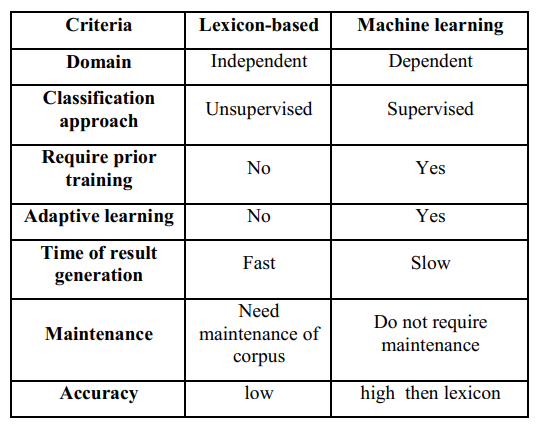
\includegraphics[width=0.5\linewidth]{images/lex_vs_ml.png}
  \caption{Comparison between lexicon and machine learning}
  \label{tab:sent_analysis_approaches}
\end{table}

Currently Sentiment analysis techniques seek to classify text as either positive, negative or neutral, using methods in Natural language processing (NLP). The common approach implemented involves statistical analysis and machine learning methods. \cite{ref2}

%
However people often express a particular emotion towards a certain topic. Specific emotions such as anger can lead to social unrest. This is undesirable but it can be helpful if we are able to quickly detect this before it occurs.
%
The proposed system will be a hybrid system it will use both machine learning approach as well as lexicon-based approach to detect both sentiment polarity and emotion.


\clearpage


\section{Methodology}
\subsection{Introduction}
In the previous chapter we explained some of the techniques which had been applied by different
researchers on sentiment analysis. We tried also to explain the short comings and
strength of each technique or method applied before this research. In this chapter we are going to
explain the software and hardware development tools which we are going to use in the
implementation and development of the geographical mood detection tool. An algorithm which
the system will follow is also going to be shown in this chapter. Timely discovery of the
sentimental or opinionated web content in our case, will help the state or the government security
in the decision making, to detect sentiment of people\textquotesingle s opinions on a given topic and  to chart the results in real-time for analysis.


\begin{figure}[h]
  \centering
  \pgfimage[width=0.8\linewidth]{images/steps_to_analyse_text}
  \caption[Steps to analyze sentiment data]%
  {Steps to analyze sentiment data}
  \label{fig:ALAP:sm1}
\end{figure}




\section{Lexicon (VaderSentiment)}
A lexicon is information about a word in a particular language. Lexicon based sentiment analysis makes use of labeled text this is very useful in detecting sentiment by emoticons. 
%
VaderSentiment is an open source library written in the python language that can be used to achieve lexical based sentiment analysis.\\ \\
VADER is specifically made to cater for sentiments expressed in social media.
VADER lexicon, are labeled in accordance to their sentiment polarity, positive, neutral or negative.
 \\ \\
An emoticon also known as "emotion icon", is a sequence of characters which are a pictorial representation of a facial expression, numbers and letters to express a person's feelings or mood, or as a time-saving method rather than to type out a whole word, an emoticon can be used to convey the writer's feelings or intended tone. \\ \\

Some key features of Vader sentiment are: -

\begin{enumerate}

\item
Punctuation: The use of an exclamation symbol(!) can increase the intensity of the sentiment but without changing the polarity of the sentiment. For example, “The weather there is good!” is more intense than “The weather there is good.” and an increase in the number of exclamations in turn increases the intensity of the sentiment accordingly.

\item
Capitalization: Making use of upper case letters adds emphasis to a sentiment-relevant word, if the sentence is written in lower case letters the upper case letters increases the intensity of the sentiment.For example, “The weather there is GREAT!” conveys more intensity than “The weather there is great!”
\item
Degree modifiers: Also known as intensifiers, they influence the sentiment magnitude  by either decreasing or increasing the intensity. For example, “The roads here are extremely good” is more intense than “The roads here are good”, whereas “The roads here are ok” decreases the intensity.
\item
Conjunctions: words like "but" are conjugation or joining words that indicate a change in the polarity of the detected sentiment of the text. “The roads here are good, but the traffic lights are horrible” has mixed sentiment, with the latter half dictating the overall rating.
\item
Preceding Tri-gram: We can examine a tri-gram of the text, at least 90\% of scenarios that involve negation can invert the polarity of the sentence. A negated sentence would be “The roads out here are not really all that good”.
\end{enumerate}

\clearpage
\subsection{Subjectivity and Objectivity (TextBlob)}
Subjectivity and objectivity differentiates opinionated and factual based text. \cite{ref2}
Being able to detect subjectivity and objectivity is an important part of sentiment analysis, because it can tell us more about the authors emotions and intentions, a subjective person is more likely to invoke action than an objective person. TextBlob python library can be used to detect the degree of subjectivity and the degree of objectivity, these results together with the polarity scores will be used to determine the impact of the sentiment. 


\subsection{Multi-label convolutional neural network text classifier (Spacy)}

SpaCy is a free, open-source library for advanced Natural Language Processing (NLP) in Python \\
Spacy makes use of a neural network text classifier. SpaCy can be used to categorize documents into the different emotion classes.
The Neural network is trained using stochastic gradient descent where the estimate of the error used to update the weights is calculated based on a subset of the training dataset. \\


\begin{figure}[h]
  \centering
  \pgfimage[width=0.7\linewidth]{images/sgd}
  \caption[Stochastic gradient descent]%
  {Stochastic Gradient decent, source: \url{https://pythonmachinelearning.pro/complete-guide-to-deep-neural-networks-part-2/}}
  \label{fig:ALAP:sm3}
\end{figure}






A SpaCy model uses statistical decisions to make predictions, the decision is based on examples used to train the model. Training the model requires training data, training data is: examples of text with the labels that we want to predict. This will be in the following categories
\begin{itemize}
\item "anger"
\item "disgust"
\item "fear"
\item "sadness"
\item "shame"
\item "joy"
\item "guilt"
\end{itemize}




The following diagram shows how SpaCy model is trained

\begin{figure}[h]
  \centering
  \pgfimage[width=0.7\linewidth]{images/spacy_training}
  \caption[SpaCy Training]%
  {SpaCy Training, source: \url{https://spacy.io/usage/training}}
  \label{fig:ALAP:sm3}
\end{figure}
 

\subsection{Training Dataset (ISEAR)}

The wheel of emotions by Robert Plutchik, shows eight primary emotions, each emotion is positioned with an opposite for example joy is the opposite of sadness, anger is the opposite of fear, trust is the opposite of disgust, and surprise is the opposite to anticipation. This group of four opposite emotion pairs forms 8 basic emotions. Plutchik's wheel also shows connections between the various emotions using a color wheel which also shows the different degrees of intensity for each emotion. The intensity of the emotion increases towards the center of the circle and decreases away from the center of the circle. For example, serenity has less intensity than joy, and ecstasy has more intensity than joy. The emotions can also be combined to form a different emotion. For example, combination of joy and trust can result in a new emotion "love". Likewise, joy, anger and trust are combined and form jealousy \cite{ref4}.

\begin{figure}[h]
  \centering
  \pgfimage[width=0.5\linewidth]{images/emotion_wheel}
  \caption[Robert Plutchik's wheel of emotions]%
  {Robert Plutchik's wheel of emotions, source: \url{https://psicopico.com/en/la-rueda-las-emociones-robert-plutchik/}}
  \label{fig:ALAP:sm3}
\end{figure}

International Survey on Emotion Antecedents and Reactions (ISEAR) is an open source texual data set collected by Klaus R. Scherer and Harald Wallbott. 
ISEAR data set contains seven major emotions based on Robert Plutchik's wheel of emotions : guilt, shame, disgust, sadness, anger, fear,  joy.\\
It has over 7,600 entries for the emotion classes. This will be a good training data set for emotion detection.
\clearpage

\subsection{Streaming twitter (tweepy)}
Tweepy is an open source python library that can be used to stream tweets from twitter in real time through the Twitter API. The twitter API can accept parameters to filter tweets based on geolocation, language and topic (i.e. tweets containing a particular word phrase or hashtag)


\subsection{Text Processing document}
Text needs to be normalized after it is obtained, text normalization includes the following steps:
\begin{itemize}
\item converting all letters to lower or upper case
\item converting numbers into words or removing numbers
\item removing punctuations, accent marks and other diacritics
\item removing white spaces
\item expanding abbreviations
\item removing stop words, sparse terms, and particular words
\item text canonicalization
\end{itemize}

We also remove numbers since they are not relevant to our analyses. We use regular expressions to remove numbers.




\subsection{Confusion matrix}
A confusion matrix is used in machine learning to determine the performance of a classification algorithm. It is a tabular form than compares test data for which its true values are known. We will use the confusion matrix to evaluate the performance of my classification model.

A confusion matrix consists of the following classes.
 \begin{itemize}

\item
true positives (TP): This is when we have given a correct positive prediction

\item
true negatives (TN): This is when we have given a correct negative prediction.

\item
false positives (FP): This is when we have predicted yes, but the true value is no

\item
false negatives (FN): This is when we have predicted no, but the true value is yes

\end{itemize}

\begin{figure}[h]
    \centering
    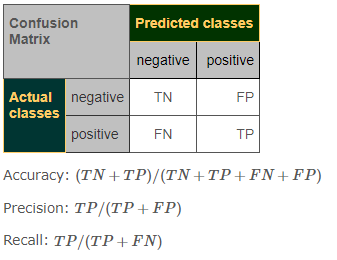
\includegraphics{images/confusion_matrix.png}
    \caption[Confusion matrix]{Confusion matrix}
\end{figure}

  The above table shows how to determine the accuracy of the prediction using a confusion matrix. However, there are problems with accuracy. It assumes equal costs for both kinds of errors that is to say it assumes that we have an equal number of positives and negatives. A 99\% accuracy can either be excellent, good, mediocre, poor or terrible depending upon the problem
\clearpage
In the case of having multiple classes the confusion matrix becomes


\begin{figure}[h]
    \centering
    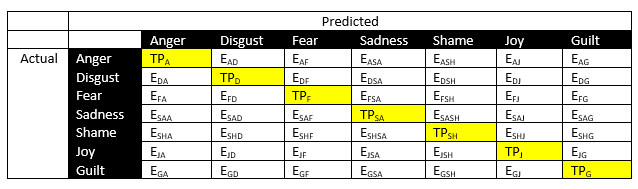
\includegraphics{images/confusion_matrix_2.png}
    \caption{Confusion matrix with multiple classes}
\end{figure}

Things to notice about a confusion matrix with multiple classes
\begin{itemize}
\item \textbf{total number of test examples} of any class if given by the sum of the corresponding row \textbf{(i.e TP + FN)}
\item \textbf{Total number of False Negatives} for a class is the sum of values in the corresponding row excluding the \textbf{True positives}

\item \textbf{Total number of false positives} for a class is the sum of values in the corresponding column excluding the \textbf{true positives}

\item \textbf{Total number of true negatives} for a certain class will be the sum of all columns and rows  excluding that classes column and row
\end{itemize}
  
\textbf{Accuracy} calculated as the sum of correct classifications divided by the total number of classifications\\
\textbf{Precision} is calculated as \textbf{ TP/(TP+ FP)}\\
\textbf{Recall} also called sensitivity, corresponds to the true positive rate of the considered class
\\
calculated as Recall=Sensitivity=TP/(TP+FN)

\clearpage



\chapter{Implementing Sentiment analysis}

\section{Introduction}
We will now outline the steps we will take to implement sentiment analysis, using some of the NLP techniques discussed.

\subsection{Implementing (VaderSentiment and TextBlob)}


Using \textbf{"VaderSentiment"} library. Using an analyzer object, and looping through the list of tweets  calling the analyser.polarity\_scores() method and appending the results to an array.

\begin{lstlisting}
from vaderSentiment.vaderSentiment import SentimentIntensityAnalyzer
analyser = SentimentIntensityAnalyzer()#create the vader sentiment analyser object
sentiment_vs_tweets=[]#array will hold the processd tweets with the sentiment and objective labels
index=0
for t in tweets:
    sentiment_vs_tweets.append( analyser.polarity_scores(t) )#add the processed tweet to the list
    print(sentiment_vs_tweets[index])#print the sentiment polarity and subjecivity
    index=index+1
\end{lstlisting}


The above code will produces the following results

\begin{lstlisting}
{'neg': 0.252, 'neu': 0.581, 'pos': 0.168, 'compound': -0.3182}
{'neg': 0.0, 'neu': 1.0, 'pos': 0.0, 'compound': 0.0}
{'neg': 0.194, 'neu': 0.806, 'pos': 0.0, 'compound': -0.5574}
{'neg': 0.0, 'neu': 1.0, 'pos': 0.0, 'compound': 0.0}
{'neg': 0.194, 'neu': 0.806, 'pos': 0.0, 'compound': -0.5574}
\end{lstlisting}




Using \textbf{TextBlob} to detect the degree of subjectivity and objectivity of the documents.


\begin{lstlisting}
#here we use TextBlob python library to detect sentence/tweet/document polarity as well as subjectivity and store the results
#textblob uses a machine learning approach
from textblob import TextBlob
sentiment_tb_tweets=[]#array will hold the processd tweets with the sentiment and objective labels
index=0
for t in tweets:
    sentiment_tb_tweets.append( TextBlob(t) )#add the processed tweet to the list
    print(sentiment_tb_tweets[index].sentiment)#print the sentiment polarity and subjecivity
    index=index+1
    
sentiment_tb_tweets[0].subjectivity
\end{lstlisting}


The above code produces the following results


\begin{lstlisting}[language=Python]
Sentiment(polarity=0.0, subjectivity=0.25)
Sentiment(polarity=0.14285714285714285, subjectivity=0.31785714285714284)
Sentiment(polarity=0.0, subjectivity=0.06666666666666667)
Sentiment(polarity=0.2, subjectivity=0.2)
Sentiment(polarity=0.0, subjectivity=0.06666666666666667)
\end{lstlisting}

\clearpage

\subsection{Training SpaCy Text classifier}
Using the ISEAR training data
We can train a SpaCy model to classify text into some categories
\begin{figure}[h]
  \centering
  \pgfimage[width=0.5\linewidth]{images/isear}
  \caption{Sample ISEAR training dataset with labels}
  \label{fig:ALAP:sm1}
\end{figure}

We begin training the SpaCy model on the above training set,
start by reading in the data 
\begin{lstlisting}
nlp    = spacy.load('en_core_web_sm')#load english model
file    = open("data/train_data.txt","r")#read in training set from text file uses pipe delimiter
#read in the training set with the labels
for row in f_data:
    train_data.append( (row.split('|')[0],\
                        {"cats":\
                         {\
                          "anger"    :int(row.split('|')[1]),\
                          "disgust"  :int(row.split('|')[2]),\
                          "fear"     :int(row.split('|')[3]),\
                          "sadness"  :int(row.split('|')[4]),\
                          "shame"    :int(row.split('|')[5]),\
                          "joy"      :int(row.split('|')[6]),\
                          "guilt"    :int(row.split('|')[7])\
                        }}) )
                        
\end{lstlisting}
\clearpage
We then update the NLP model with the new training set
\begin{lstlisting}
#create the spacy nlp pipeline
textcat = nlp.create_pipe('textcat')
#add the pipeline to the nlp model| last=true since we want to add these conponents at the end of the model
nlp.add_pipe(textcat, last=True)
#declare the lables/categories
textcat.add_label('anger')
textcat.add_label('disgust')
textcat.add_label('fear')
textcat.add_label('sadness')
textcat.add_label('shame')
textcat.add_label('joy')
textcat.add_label('guilt')

optimizer = nlp.begin_training()
#next we will update the model with our own train_data from the csv file
for itn in range(1):
    for doc, gold in train_data:
        random.shuffle(train_data)
        losses = {}
        index = 0
        for text, annotations in train_data:
            nlp.update([doc], [gold], sgd=optimizer, drop=0.45, losses=losses)#drop rate at .45
            print("Iteration: {0}, %{1:.2f} Complete".format((itn+1), index/len(train_data) * 100))#show the progress
            index += 1
        print(losses)
 
\end{lstlisting}


After training the model we can now run some tweets via the model 
\begin{lstlisting}
#determine the class of the tweets using the spacy model trained earlier
#create a document and run it thru the nlp pipeline 
classified_tweets = []#array will hold the spacy classified tweets
index=0
for t in tweets:
    classified_tweets.append(  nlp(t) )
    print( classified_tweets[index].cats )#print the categories/classes of the document
    index=index+1  
\end{lstlisting}

The above code produces the following results
\begin{lstlisting}
{'anger': 0.8638094067573547, 'disgust': 0.41107258200645447, 'fear': 0.007243141997605562, 'sadness': 0.04211084172129631, 'shame': 0.7023115158081055, 'joy': 0.6675902605056763, 'guilt': 0.9010916352272034}
{'anger': 0.7449342012405396, 'disgust': 0.4830150306224823, 'fear': 0.016353892162442207, 'sadness': 0.2870638370513916, 'shame': 0.40636202692985535, 'joy': 0.1324012577533722, 'guilt': 0.41464924812316895}
{'anger': 0.7480689883232117, 'disgust': 0.4755619764328003, 'fear': 0.035106029361486435, 'sadness': 0.1592441201210022, 'shame': 0.4828783869743347, 'joy': 0.16910341382026672, 'guilt': 0.4793942868709564}
{'anger': 0.7859129905700684, 'disgust': 0.47182315587997437, 'fear': 0.026509756222367287, 'sadness': 0.32458046078681946, 'shame': 0.12689484655857086, 'joy': 0.23759214580059052, 'guilt': 0.9908844828605652}
{'anger': 0.7480689883232117, 'disgust': 0.4755619764328003, 'fear': 0.035106029361486435, 'sadness': 0.1592441201210022, 'shame': 0.4828783869743347, 'joy': 0.16910341382026672, 'guilt': 0.4793942868709564}
\end{lstlisting}

SpaCy model is able to classify the class of the text based on our training set



\clearpage

\subsection{Streaming twitter API(Tweepy)}

The python library tweepy can support accessing Twitter tweets via both Basic Authentication and OAuth. The API parameters allow filtering tweets based on language, geolocation and tweets containing a particular word or phrase.

\begin{lstlisting}
auth   = OAuthHandler(consumer_key, consumer_secret)
auth.set_access_token(access_token, access_token_secret)

stream = Stream(auth, listner)
#run this code async 
streamer=stream.filter(track=search_terms,is_async=True,languages=langs,locations=loca_tions)
\end{lstlisting}

The listener object is a class that inherits from StreamListener class, it listens for any incoming tweets, cleans the tweets and then stores them in an array.

\begin{lstlisting}
class StdOutListener(StreamListener):
    def on_data(self, data):
        obj = json.loads(str(data))#convert the tweet into a json format
        #clean the tweets before inserting into the array
        clean_tweet = remove_pattern(obj["text"],"@[\w]*")#remove twitter handles (@user)
        clean_tweet = clean_tweet.replace("[^a-zA-Z#]", " ")#replace puntuation marks
        clean_tweet = clean_tweet.replace("RT :","")#replace the re tweet symbol
        clean_tweet = re.sub('http[s]?://(?:[a-zA-Z]|[0-9]|[$-_@.&+]|[!*\(\),]|(?:%[0-9a-fA-F][0-9a-fA-F]))+', '', clean_tweet, flags=re.MULTILINE)#remove hyperlinks
        
        score       = vs_analyser.polarity_scores(clean_tweet)
        sentiment_polarity_scores.append( float(score["compound"]) )#append the sentiment score to the array
        sentiment_tb_tweets.append( TextBlob(clean_tweet) )#append the texblob object to the array
        sentiment_vs_tweets.append( nlp(clean_tweet) )#append the vader sentiment object to the array
        tweets.append(clean_tweet)#append the clean tweet to the list of tweets
\end{lstlisting}



%%%%%%%%%%%%%%%%%%%%%%%%%%%%%%%%%%%%%%%%%%%%%%%%%%%%%%%%%%%%%%%%%%%%%%%
\subsection{Evaluating SpaCy classification model}
Because of the huge size of the training dataset, using the whole data set to train and evaluate the model would take too long. The solution therefore is to use a small sample of the dataset to train and evaluate.
The training set has 23 samples and the evaluation set has 8 samples.\\
The following is the results of the evaluation based on the confusion matrix.

\begin{lstlisting}
Accuracy:  1.4285714285714286



Precision_anger:  0.6666666666666666
Precision_disgust:  1.0
Precision_fear:  0.4
Precision_sadness:  1.0
Precision_shame:  1.0
Precision_joy:  1.0
Precision_guilt:  1.0
Total_Precision:  0.8666666666666666



Recall_anger:  1.0
Recall_disgust:  0.6666666666666666
Recall_fear:  1.0
Recall_sadness:  0.5
Recall_shame:  0.5
Recall_joy:  0.5
Recall_guilt:  0.5
Total_Recall:  0.6666666666666666
\end{lstlisting}

The results for each individual classification is quite satisfactory, considering that the training set and evaluation set is considerably small. However both the total precision and the total Recall is at least 66\% this is quite satisfactory.


\section{System design}

\textbf{Purpose}\\
This section describes the software design and the architecture of the geographical mood detection and tool.

\textbf{Scope}\\
This mood detection and prediction tool will help in estimating a group of social media users'
mood toward specific topics in terms of their sentiments and opinions from their posts on twitter.

\textbf{System overview}\\

To come up with the geographical mood detection tool we utilize open source libraries, and open datasets to create models, and analyze the text then detect the mood. We will graph the results in real time then monitor the plots. From the plots we can visualize the polarity, subjectivity and emotion. We can monitor the sentiment trends in real time.

\subsection{Architectural Design}
The geographical mood detection tool, takes into consideration a number of aspects to achieve the goal namely: The sentiment polarity, degree of subjectivity, and the emotion classification. The graphical presentation of the whole system and methods to be followed are shown below:

\begin{figure}[h]
  \centering
  \pgfimage[width=0.8\linewidth]{images/system_overview}
  \caption[System Architecture]%
  {System Architecture}
  \label{fig:ALAP:sm1}
\end{figure}


The first four modules describe the process implemented in order to detect mood (i.e. emotions,
speculations, evaluations and opinions) of a group of social media users through sentiment
analysis. The extracted sentiments will then help in predicting action from the group of social
media users.

\subsection{Sentiment Analysis (detection and classification)}
Once the collected corpus is clean, VaderSentiment library can be used to detect sentiment polarity the degree of positivity or negativity. Textblob library can be used to detect the degree of subjectivity or objectivity of the tweet. And SpaCy library will be used used clasisfy the emotion of the tweet.

\begin{figure}[h]
  \centering
  \pgfimage[width=0.5\linewidth]{images/sentiment_analysis_dfd}
  \caption[Sentiment Analysis data flow diagram]%
  {Sentiment Analysis data flow diagram}
  \label{fig:ALAP:sm1}
\end{figure}


\subsection{Sequence Diagram}
The Sequence Diagram below models the collaboration of objects based on a time sequence.
It shows how the objects interact with others in a particular scenario of a use case.

\begin{figure}[h]
  \centering
  \pgfimage[width=0.5\linewidth]{images/sequence_diagram}
  \caption[Illustration of the Sequence diagram]%
  {Illustration of the Sequence diagram}
  \label{fig:ALAP:sm1}
\end{figure}


\subsection{Use Case Diagrams}
\textbf{Blogger}\\
Bloggers from all over the world interact through social media platforms by commenting and
uploading posts part of our tool\textquotesingle s task is to crawl on these platforms for text related to a searched term. 



\begin{figure}[h]
  \centering
  \pgfimage[width=0.5\linewidth]{images/use_case_blogger}
  \caption[Blogger use case diagram]%
  {Blogger use case diagram}
  \label{fig:ALAP:sm1}
\end{figure}

\clearpage
\textbf{User}\\
A user of the system may input a \textbf{keyword/phrase} that will be searched on the social media platforms which will help in mining content concerning the searched keyword. Furthermore, user has the
flexibility of changing keyword search parameters.

\begin{figure}[h]
  \centering
  \pgfimage[width=0.5\linewidth]{images/system_user_use_case}
  \caption[System user use case diagram]%
  {System user use case diagram}
  \label{fig:ALAP:sm1}
\end{figure}



\section{Development Tools}

\subsection{SpaCy}

\begin{minipage}{0.68\textwidth}
SPaCy is an open source python library used for common NLP tasks. The library implements statistical neural network models, it has language support for English, German, Spanish, Portuguese, French, Italian, Dutch as well as tokenizations for various other languages.
\end{minipage}%
%
\begin{minipage}{0.3\textwidth}
  \hspace*{.4cm}
  
\includegraphics[width=\textwidth]{images/spacy_logo}
\end{minipage}




\subsection{VaderSentiment}

\begin{minipage}{0.68\textwidth}
VaderSentiment is a python library built on top of NLTK. it is a rule-based sentiment analysis engine, and implements grammatical and syntactical rules to detect sentence polarity, positive, negative and neutral.
\end{minipage}%
%
\begin{minipage}{0.3\textwidth}
  {\ ~}\hfill
  
\includegraphics[width=.8\textwidth]{images/VaderSentiment_logo}
\end{minipage}



\subsection{TextBlob}

\begin{minipage}{0.68\textwidth}
TextBlob is a python library for processing textual data. TextBlob can be used to determine the degree of subjectivity or objectivity in a textual document.
It exposes a concise API for carrying diving into common natural language processing (NLP) tasks such as part-of-speech tagging, noun phrase extraction, sentiment analysis, classification, translation, and more.\cite{ref43}
\end{minipage}%
%
\begin{minipage}{0.3\textwidth}
  \hspace*{.4cm}
  
\includegraphics[width=\textwidth]{images/textblob_logo}
\end{minipage}


\subsection{Jupyter Notebook}

\begin{minipage}{0.68\textwidth}
The Jupyter Notebook App is a server-client application that allows editing and running notebook documents via a web browser. The Jupyter Notebook App can be executed on a local desktop requiring no internet access or can be installed on a remote server and accessed through the internet.

\end{minipage}%
%
\begin{minipage}{0.3\textwidth}
  \hspace*{.4cm}
  
\includegraphics[width=\textwidth]{images/jupyter_notebook}
\end{minipage}


\subsection{MatplotLib}

\begin{minipage}{0.68\textwidth}

Matplotlib is a plotting library for the Python programming language and its numerical mathematics extension NumPy. It provides an object-oriented API for embedding plots into applications using general-purpose GUI toolkits like Tkinter, wxPython, Qt, or GTK+.
\end{minipage}%
%
\begin{minipage}{0.3\textwidth}
  \hspace*{.4cm}
  
\includegraphics[width=\textwidth]{images/matplot_lib}
\end{minipage}


\section{Creating Twitter Application}

Navigate to the url \url{https://developer.twitter.com/en}\\
under the "App Details" tab fill in your application details and move to the next tab "Keys and Tokens"

\begin{figure}[h]
  \centering
  \pgfimage[width=0.6\linewidth]{images/twitter_1}
  \caption[Application Details]%
  {Application Details}
  \label{fig:ALAP:sm1}
\end{figure}

Collect the keys, secret key and API key which will be used by the tweepy library for authentication and streaming tweets.


\begin{figure}[h]
  \centering
  \pgfimage[width=0.6\linewidth]{images/twitter_2}
  \caption[Access keys]%
  {Access keys}
  \label{fig:ALAP:sm1}
\end{figure}

\clearpage
Set the permissions for your API key.


\begin{figure}[h]
  \centering
  \pgfimage[width=0.5\linewidth]{images/twitter_3}
  \caption[API permissions]%
  {API permissions}
  \label{fig:ALAP:sm1}
\end{figure}



\section{Implications of findings}

The boom in the availability of opinionated and emotionally charged data from various review sites, RSS feeds, and social networks has created a wave of interest in sentiment analysis by both academia and businesses.
%
This is because there are many practical and potential applications of sentiment analysis. A Geographical Mood Detection tool can assist organizations and service providers to know the mindset of the people they are working with for instance:\\

\textbf{Business Applications}\\
The tool can be adopted by any business which would like the ability to exploit unstructured data for actionable insights. Potential applications would be extracting product review, brand tracking, modifying
marketing strategies and mining financial news.\\

\textbf{Politics}\\
Sentiment analysis enables tracking of opinion on issues and subjectivity of bloggers in
political blogs. Sentiment analysis can help political organization to understand which issues
are close to the voter\textquotesingle s heart.\\

\textbf{Government Intelligence}\\
For efficient rule making, the tool can be used to assist in automatically analyzing the opinions of
people about pending policies or government-regulation proposals. Other applications include
tracking the citizen\textquotesingle s opinion about a new scheme, predicting the likelihood of the success of a new legislative reform to be introduced and gauging the mood of the public towards a scandal
or controversy.


\chapter{Recommendations, future work and conclusion}


\section{Recommendations}

This tool may be used by the government, Non-Governmental Organizations, and business corporations. Investors may need to analyze the environment first before starting a business
venture, hence detecting mood of a society concerning a particular topic/product is of vital importance.
We also propose that the tool can be used with experts in the field of big data analytics so as to gain
better insights into their business/political atmosphere. It is clear that the adoption of advanced analytic approaches such as those used by our tool can guide organizations to  strategize and help them to make smarter decisions.\\

\section{Future Work}
In future work we plan to devise an approach to further improve the accuracy of mood detection by including not only textual information but also pictorial, video, and audio classification.
Having said that, we believe that sentiment analysis will only increase in importance as more and
more people use online channels to communicate, both directly and indirectly.
We also plan to consider the issue of sarcasm, that is, sarcastic sentences express negative opinion
about a target using positive words. For example:\\

$\cdot$ “Nice perfume. You must marinate in it”.\\
The sentence contains only positive words, yet still, it expresses a negative sentiment.






\chapter{Results and analysis}\label{ch:Results}

\section{Data visualization}

The human brain processes information in a visual way, therefore it makes more sense to display the information using charts and graphs to visualize the information, as opposed to dumping large amounts of data onto spread sheets and reports. Data visualization makes it easier to identify areas that need attention.

\subsection{matplotlib and seaborn}

Seaborn is a Python data visualization library based on matplotlib. It provides a high-level interface for drawing attractive and informative statistical graphics.
Matplotlib allows plotting multiple graphs on a single figure. Analysis can be made on different metrics at the same time. It also allows updating graph data in real-time.

\begin{figure}[h]
  \centering
  \pgfimage[width=0.5\linewidth]{images/graphs_results}
  \caption[Real time plot of the analysis]
  {Real time plot of the analysis}
  \label{fig:ALAP:sm1}
\end{figure}


The \textbf{word-cloud} gives a summary of the tweets in real-time.\\
The \textbf{time-series} gives a \textbf{stochastic trend} of the polarity of the tweets, with \textbf{1 = positive, -1 = negative and 0 = neutral}.
The \textbf{bar chart} displays the values of the number of tweets in the given category\\
The \textbf{heat map} shows the \textbf{polarity} as well as the \textbf{subjectivity} in terms of percentage,
a negative and subjective scenario is the least desirable while a positive and objective scenario is the most desirable.\\

With this real-time analysis one can quickly see the prevailing mood as well as a summary of the tweets around a given topic.





\chapter{Conclusion}

This research project has examined the role of social media networks in determining people's mood based on textual information they post. We developed a geographic mood detection tool based on social media.

The results show that by utilizing social media platforms e.g. twitter, a tool can actually analyze people's mood towards a subject and inform the relevant authorities in real-time to know what the people\textquotesingle s general mood towards a particular subject is.

Making use of open python libraries and training data sets we were able to classify the general mood 
of people based on their geographical location.

Furthermore, this tool can be adopted by businesses, organizations and politicians who would like to have an edge and an insight into people's opinions over a giver topic.



